\section{Resultados}
Los experimentos se ejecutaron con el script \texttt{main\_benchmark.py}, que registra el tiempo de ejecuci\'on y el error $L_2$ de cada m\'etodo. En la Tabla~\ref{tab:benchmark} se resumen los valores obtenidos.

\begin{table}[h]
\centering
\begin{tabular}{lcc}
\hline
M\'etodo & Tiempo (s) & Error $L_2$\\
\hline
FTCS & 0.165 & 4.1e-02\\
9 puntos & 0.178 & 3.3e-02\\
(1,13) & 0.339 & 8.7e-06\\
\hline
\end{tabular}
\caption{Comparaci\'on de tiempo de ejecuci\'on y error.}
\label{tab:benchmark}
\end{table}

La Figura~\ref{fig:time-error} muestra la relaci\'on entre el tiempo de c\'omputo y el error de cada m\'etodo, mientras que la Figura~\ref{fig:contour} presenta el contorno de temperatura obtenido con el esquema de trece puntos. El m\'etodo \emph{(1,13)} es el m\'as preciso pero tambi\'en el m\'as costoso, en tanto que FTCS resulta el m\'as r\'apido.

\begin{figure}[h]
\centering
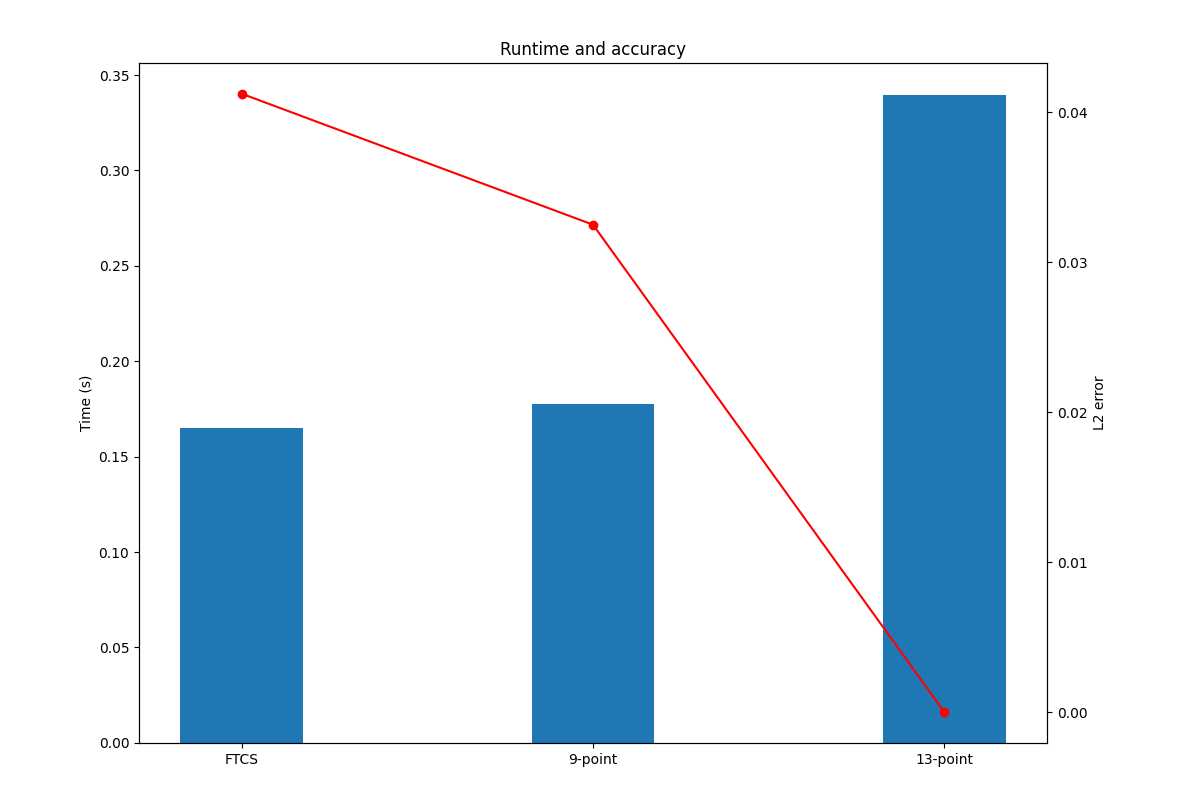
\includegraphics[width=0.7\linewidth]{resultados/Figure_1.png}
\caption{Tiempo de ejecuci\'on frente a error $L_2$.}
\label{fig:time-error}
\end{figure}

\begin{figure}[h]
\centering
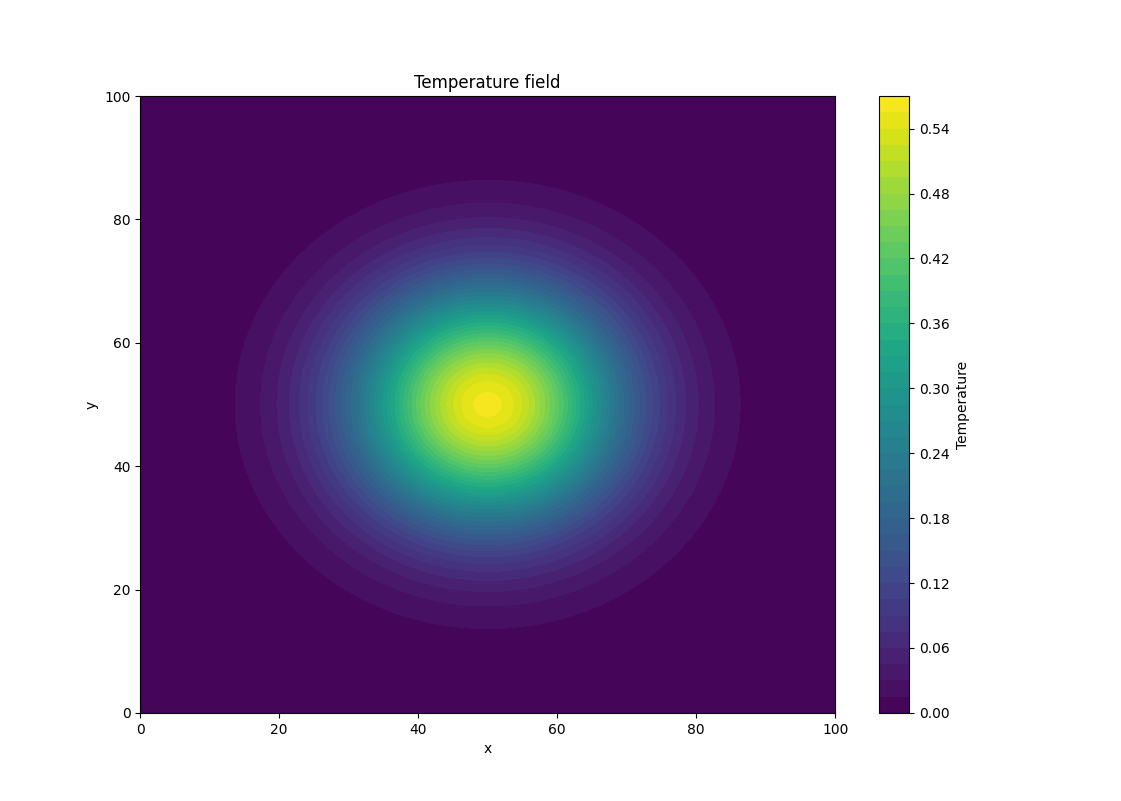
\includegraphics[width=0.7\linewidth]{resultados/Figure_2.png}
\caption{Contorno de temperatura calculado con el esquema de trece puntos.}
\label{fig:contour}
\end{figure}
